\documentclass{beamer}

\usepackage[main=english,finnish]{babel}
\usepackage{cmbright}
\usepackage{fontspec}
\usepackage{booktabs}
\usepackage{pifont}
\usepackage{dot2texi}
\usepackage{amsmath}

\newsavebox{\mysavebox}
\newlength{\myrest}

\DeclareMathOperator*{\argmax}{arg\,max}
\newcommand{\cmark}{\textcolor{red}{\ding{51}}}%
\newcommand{\xmark}{\textcolor{green}{\ding{55}}}%
\newcommand{\mtag}[1]{% \tag{<name>}
\mathchardef\mhyphen="2D % Define a "math hyphen"
\ensuremath{\langle{}#1\rangle{}}}
%\usepackage{polyglossia}
\setsansfont[Ligatures = TeX,
             BoldFont  = CMU Bright SemiBold,
             ItalicFont = CMU Bright Oblique,
            ]{CMU Bright Roman}
\setmainfont[Ligatures = TeX,
             BoldFont  = CMU Bright SemiBold,
             ItalicFont = CMU Bright Oblique,
            ]{CMU Bright Roman}
\setmonofont[Ligatures = TeX,
             BoldFont  = CMU Typewriter Text Bold,
             ItalicFont = CMU Typewriter Text Oblique,
            ]{CMU Typewriter Text}
\usetheme{Madrid}

\mode<presentation>
\setbeamercovered{transparent}
\setbeamertemplate{enumerate items}[default]
\setbeamertemplate{itemize items}[default]

\title[POS tagger internals]{Apertium part-of-speech tagger internals}
\institute[JYU]{University of Jyväskylä\\
\vspace{5mm}
\url{https://www.github.com/frankier/tagger-internals-slides/}}
\author[Frankie Robertson]{Frankie Robertson\texorpdfstring{\\
\href{mailto:frrobert@student.jyu.fi}{\texttt{frrobert@student.jyu.fi}}}{}}

\date{18th of July, 2016}

\titlegraphic{\vfill\includegraphics[height=1.5cm]{null.pdf}
  \hfill
  \includegraphics[height=1.5cm]{jyu.pdf}
}

\begin{document}

\section{Title}
\begin{frame}
  \titlepage{}
\end{frame}

\section{Orientation}
\begin{frame}
\frametitle{Orientation}
\hspace*{-5mm}
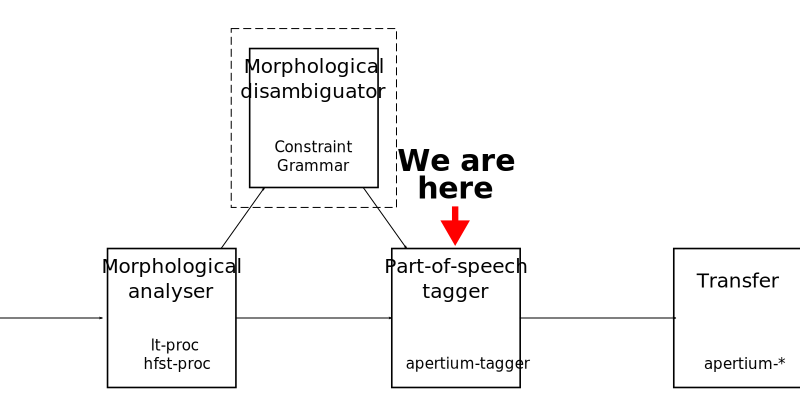
\includegraphics[width=\paperwidth]{we-are-here.pdf}
\end{frame}

\begin{frame}
\frametitle{An idealised part-of-speech tagger}
\begin{columns}
  \begin{column}{4cm}
    \includegraphics[width=4cm]{time-travelling-linguist.png}
  \end{column}
  \begin{column}{8cm}
    \begin{itemize}

      \item Hard-working linguist picks the correct morphological analysis of
        every sentence that ever has been or will be.

      \item Tagger looks up all the analyses of our input sentence. Outputs the
        most frequent analysis of each word.

      \item $\argmax_{t_i\in{}T}{P(t_i|w_0,w_1,\ldots,w_n)}$

      \item ``Pick the most likely tag for the word in the context of the
        sentence''

    \end{itemize}
  \end{column}
\end{columns}
\end{frame}

\begin{frame}
\frametitle{Not so ideal}
\begin{itemize}

  \item This is impossible. Instead our linguist works for a while and comes
    back with a tagged corpus of 10\,000 sentences.

  \item If the sentence to tag isn't in our corpus, the previous algorithm
    can't do anything. Our tagger must deal with data sparsity.

  \item If the sentence is in our corpus once, it could be tagged with a rare
    interpretation. Our tagger shouldn't overfit.

  \item How? Reduce the number of parameters and smooth over incomplete data.

\end{itemize}
\end{frame}

\section{Simple taggers}
\begin{frame}
\frametitle{A zero-parameter, zero-gram model}
\begin{itemize}

  \item Assume that all tags are uniformly distributed independently from
    context.

  \item Since they are evenly distributed, we can just pick the first one.

  \item Usually implemented with Apertium as \texttt{cg-proc -1}.

  \item This is our baseline.

\end{itemize}
\end{frame}

\begin{frame}
\frametitle{Unigram tagger}
\begin{itemize}

  \item In general, discard all context apart from the word itself.

  \item $\argmax_{t_i\in{}T}{P(t_i|w_i)}$

  \item In Apertium, result of a Google Code-In project by m5w based on
    \url{http://coltekin.net/cagri/papers/trmorph-tools.pdf} --- Supervised
    (needs a tagged corpus).

  \item Model one: Just pick the most frequent whole analysis. So if our corpus
    is just $work\mtag{n}\mtag{sg}$ once and $work\mtag{vblex}\mtag{imp}$ zero
    times our tagger always picks $work\mtag{n}\mtag{sg}$. If a word isn't in
    our corpus at all this acts like the zero-gram case due to smoothing
    (``cross fading'' between different models).

  \item Model two: decompose using Bayes' theorem: $P(t) = P(root, analysis) =
    P(root|analysis)P(analysis)$. So count each analysis string and count for
    each analysis how many of each roots it has to estimate. From previous
    example, our model can now tag an unseen word as $\mtag{n}\mtag{sg}$.

\end{itemize}
\end{frame}

\section{Coarse tags}
\begin{frame}
\frametitle{From analyses to coarse tags and ambiguity classes}
\begin{columns}
  \begin{column}{4cm}
    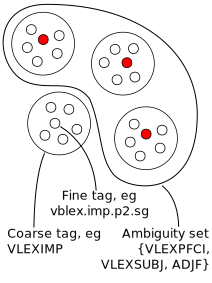
\includegraphics[width=4.5cm]{fine-coarse-ambgsets.pdf}
  \end{column}
  \begin{column}{8cm}
    \begin{itemize}

      \item Cluster morphological analyses into coarse tags --- reduces number
        of parameters.

      \item $coarsen \colon Analysis \rightarrow Coarse\ Tag$;\\
        $coarsen(\mathrm{di\mtag{vblex}\mtag{imp}\mtag{p2}\mtag{sg}})\linebreak = VLEXIMP$

      \item $coarsen\hbox{-}many \colon Analyses \rightarrow Ambiguity Set$;\\
        $coarsen\hbox{-}many(\allowbreak{}\{
          work\mtag{n}\mtag{sg},
          work\mtag{vblex}\mtag{imp}\})\linebreak = NOUNSG, VBLEXIMP$\\

      \item $discriminate \colon Analyses, Coarse Tag \rightarrow Analysis $;
        $discriminate(\{work\mtag{n}\mtag{sg},\allowbreak\work\mtag{vblex}\mtag{imp}\}, NOUNSG) = work\mtag{n}\mtag{sg}$\\

      \item $coarsen\hbox{-}many$ and $discriminate$ can be implemented in terms of $coarsen$.

    \end{itemize}
  \end{column}
\end{columns}
\end{frame}

\begin{frame}
\frametitle{The reduced morphological disambiguation problem}
\begin{itemize}

  \item First run, $coarsen\hbox{-}many$ for each incoming token to get a
    stream of ambiguity classes.

  \item Then, run our coarse tagging tagger on the ambiguity classes to get a
    coarse tag for each token.

  \item Then, run $discriminate$ on each tag in the resulting coarse tag stream
    to get stream of disambiguated morphological analyses.

  \item Coarse tags are defined by globbing (pattern matching) fine tags and
    sometimes additionally by listing lemmas.

  \item This scheme deals with multiwords (tokens made of a series of
    (lemma, fine tags) pairs, eg compound words) by assigning a tag for the
    whole token, usually made by combining other coarse tags eg maan-kamera is
    made up of a NOUNGEN followed by a NOUNSG so we make a new tag,
    NOUNGEN\_NOUNSG.

\end{itemize}
\end{frame}

\begin{frame}
\frametitle{Picking coarse tags}
\begin{itemize}

  \item Currently you need to define coarse tags for your language in a tsx
    file.

  \item \url{https://github.com/jimregan/tag-clusterer} is a wrapper around
    \texttt{mkcls}\footnote{More info at
    \url{http://statmt.blogspot.fi/2014/07/understanding-mkcls.html}} which
    picks coarse tags for you based on a corpus.

  \item $mkcls$ maximises $P(x_i|coarsen(x_i))$: the probability
    we can guess the correct analysis given a coarse tag. Usually it should be
    possible to get this value near 1 ($\Rightarrow$ the $discriminate$ step is
    reliable).

  \item This program also tries to maximise
    $P(coarsen(x_i)|coarsen(x_{i-1}))$: the probability we can predict
    a coarse tag from a previous coarse tag. Very common lemmas sometimes
    end up with their own coarse tag.

\end{itemize}
\end{frame}

\section{Coarse tag taggers}
\begin{frame}
\frametitle{Coarse tags unigram tagger (not in Apertium)}
\begin{itemize}

  \item Not in Apertium --- explained here to help motivate what follows.

  \item Estimate $P(tag|ambiguity\hbox{-}class)$.

  \item Model consists of triples:
    $(ambiguity\hbox{-}class,\allowbreak tag,\allowbreak
    occurrence\hbox{-}count)$.

  \item Supervised training: Inspect each tagged token and increment
    $occurrence\hbox{-}count$ in the corresponding triple.

  \item Tagging: For each input ambiguity class, pick the $tag$
    with the highest $occurrence\hbox{-}count$.

\end{itemize}
\end{frame}

\begin{frame}
\frametitle{Hidden Markov Model bigram tagger}
\begin{itemize}

  \item Now we use the tag the previous word has received as context. We
    now try to estimate
    P(current\hbox{-}tag|previous\hbox{-}tag) --- the
    transition probabilities.

  \item The actual tags are the hidden part of the model.

  \item We can observe the ambiguity class --- HMM jargon: they are ``emitted''
    by the model.

  \item $P(ambiguity\hbox{-}class|tag)$ (conditional inverted from previous slide)
    is the emission probabilities.

\end{itemize}
\end{frame}

\begin{frame}
\frametitle{Diagram + intuition of tagging process}
\begin{center}
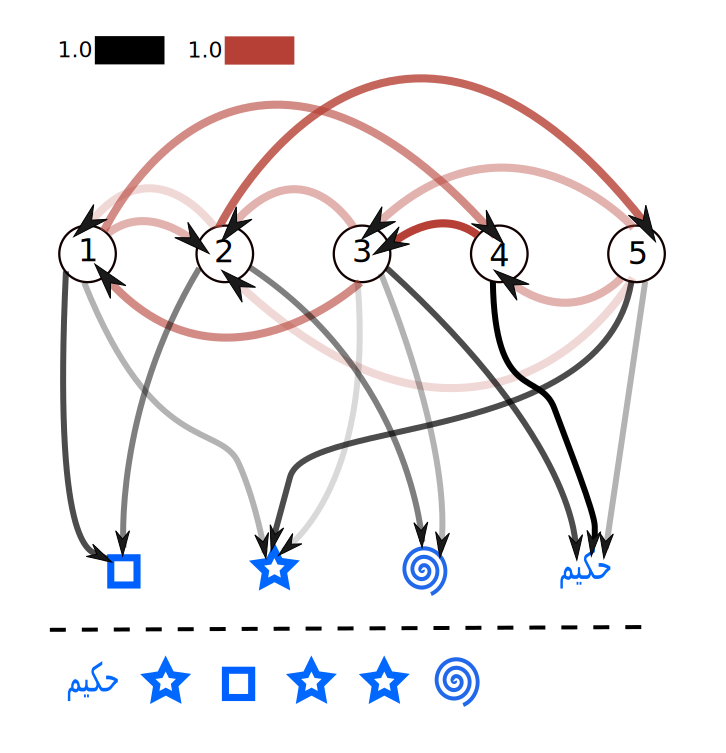
\includegraphics[height=8cm]{hmmdiagram.pdf}
\end{center}

\end{frame}

\begin{frame}
\frametitle{Viterbi tagging algorithm}
\begin{itemize}

  \item Keep track of the path probabilities through the Markov model.

  \item At an unambiguous token, backtrack and output the tags we've
    remembered.

  \item First step, set the probability of a sentinel tag to 1: $V_{1,START} = 1$

  \item At step $n$ for each possible $tag$ we calculate $V_{n,tag}$

  \item We consider each prev\hbox{-}tag (from all possible previous tags S),
    \[\hspace{-0.5cm}V_{n,tag} &=& \max_{prev\hbox{-}tag \in S} \left(  P( ambg\hbox{-}class | tag ) \cdot P (tag | prev\hbox{-}tag) \cdot V_{n-1,prev\hbox{-}tag}\right)\]

  \item At each step $n$ for each $tag$ we save the value of the
    $prev\hbox{-}tag$ for use during backtracking.

\end{itemize}
\end{frame}

\begin{frame}
\frametitle{Training}
\begin{itemize}

  \item Supervised training: just estimate the probabilities with their frequency
    in the corpus.

  \item Unsupervised training using Baum-Welch. Idea: iteratively improve our
    model to maximise the probability of the observations in our untagged
    corpus. We ``fit our model to our data''.

\end{itemize}
\end{frame}

\begin{frame}
\frametitle{Lightweight Sliding Window Part of Speech Tagger (LSWPoST)}
\begin{itemize}

  \item Based on work in 2005 by Sanchez-Villamil, M. L. Forcada, and R. C.
    Carrasco.

  \item In Apertium, considers a context of the previous and next tag.

  \item It estimates the best tag by summing all possible
    $P((prev\hbox{-}tag,tag,next\hbox{-}tag)|(prev\hbox{-}ambg\hbox{-}class,tag,next\hbox{-}ambg\hbox{-}class))$
    (no search/decoding process)

  \item Unsupervised learning of these probabilities by an iterative process.

  \item Paper at \url{http://arxiv.org/pdf/1509.05517v1.pdf}.

\end{itemize}
\end{frame}

\section{End bits}
\begin{frame}
\frametitle{Comparison}
\begin{itemize}

  \item For Catalan:

  \begin{table}
  \begin{tabular}{ll}
    Model & Per token accuracy (\%)\\
    \toprule
    0-gram & 86.50\\
    Bigram unsupervised & 91.51±1.16\\
    LSWPoST & 92.99±0.84\\
    Unigram model 1 & 93.86±1.13\\
    Unigram model 2 & 93.90±1.09,\\
    Bigram supervised & 96.00±0.87.
  \end{tabular}
  \end{table}

  \item Take with a pinch of salt. Per token means includes full stops. If we
    have sentences 20 tokens long: 86.5\% token accuracy means 5.4\% sentence
    rate, 96\% accuracy means 44.2\% sentence rate.

  \item A lot more info available at \url{http://wiki.apertium.org/wiki/Comparison_of_part-of-speech_tagging_systems}

\end{itemize}
\end{frame}

\begin{frame}
\frametitle{Comparison cont.}
\begin{table}
\begin{tabular}{llll}
  Model & untagged crp & tagged crp & tsx \\
  \toprule
  0-gram & \xmark & \xmark & \xmark\\
  Unigram & \xmark & \cmark & \xmark\\
  Bigram unsup & \cmark & \xmark & \cmark\\
  LSWPoST & \cmark & \xmark & \cmark\\
  Bigram sup & \xmark & \cmark & \cmark\\
\end{tabular}
\end{table}
\begin{itemize}

\end{itemize}
\end{frame}

\begin{frame}
\frametitle{My work on the tagger}
\begin{itemize}

  \item In process GSOC project trying to improve apertium-tagger in two
    directions.

  \item Experimenting with different ways to integrate lt-proc output and CG
    disambiguated output into the current tagger training and tagging
    processes.

  \item A new tagger based on the generalised perceptron aiming to:
    \begin{itemize}
      \item Improve accuracy rates over the bigram tagger for supervised
        tagging.
      \item Provide a usable tagger for languages where writing a complete tsx
        ranges from very annoying to infeasible, e.g. Turkic languages
      \item Possibly in the process provide a more usable tagger for other languages too.
      \item Allow user configuration over which features within the sentence
        are used for disambiguating tokens, and which parts of a candidate token to
        consider important for disambiguation.
    \end{itemize}

\end{itemize}
\end{frame}

\begin{frame}
\frametitle{Further reading}
\begin{itemize}

  \item See the links throughout the presentation (these slides are available
    at \url{https://www.github.com/frankier/tagger-internals-slides/})

  \item At \url{https://www.github.com/frankier/apertium-hmm2dot} there are
    some tools I made to explore some of the tagger internals. This includes a
    tool to visualise bigram HMM tagger models, tools to show what's inside a
    tagger model file, and tools to show the input streams to the taggers.

  \item Read the source code

\end{itemize}
\end{frame}

\end{document}
